
%Titulo:
% Modelos para localizaci�n de ajustadores de accidentes automovil�sticos
%Abstract:
% En este trabajo se intentan establecer pol�ticas de ubicaci�n
% de ajustadores de accidentes automovil�sticos
% con el fin de atender a los usuarios en el menor tiempo posible.
% Se presentar�n modelos de programaci�n entera mixta, 
% en los cuales se considera, por un lado,
% la asignaci�n fija de bases a cada ajustador,
% y por otro, asignaciones din�micas y pol�ticas de re-despliegue.

\documentclass[10pt,usenames,dvipsnames,svgnames,table]{beamer}
\usetheme{Warsaw}
\usepackage[english]{babel}
\usepackage[latin1]{inputenc}

\usepackage{graphicx}
\usepackage{epstopdf}
\graphicspath{ {./imagenes/} }
\title{Models for locating car wreck adjusters}
\subtitle{ENOAN 2015}
\author{Luis Maltos}
\institute[Universidad Aut\'onoma de Nuevo Le\'on]{
  Posgrado en Ingenier\'a de Sistemas \\
  FIME / UANL}

\date[ENOAN 2015]{September 2015}

\begin{document}
\begin{frame}
  \titlepage
\end{frame}

\begin{frame}{Contenidos}
  \tableofcontents
\end{frame}


%En ella se deben exponer brevemente pero con absoluta claridad, 
% la novedad y actualidad del tema,
% el objeto de la investigación,
% sus objetivos,
% la hipótesis de trabajo,
% el fundamento metodológico y
% los métodos utilizados para realizar el trabajo de investigación.
%Es decir, que la introducción es la fundamentación científica de la tesis en forma resumida.

\section{Introduction}
\begin{frame}

  The aim of this work is to support decision making regarding
  the location and redeployment of insurance agents to attend car wrecks.

  The idea is to develop models and methods for 
  (a) improving the service offered by insurance agents, 
  helping them arrive to the accident sites sooner, and 
  (b)  determining the number of adjusters required to perform 
  the service within the desired standards.

\end{frame}

\subsection{Problem}
\frame{
  \textit{The main goal is to determine the optimal bases (locations) 
    for placing the insurance company adjusters, 
    so as to minimize the average or maximum response time
    from customer calls when accidents occur.}
  \begin{center}
    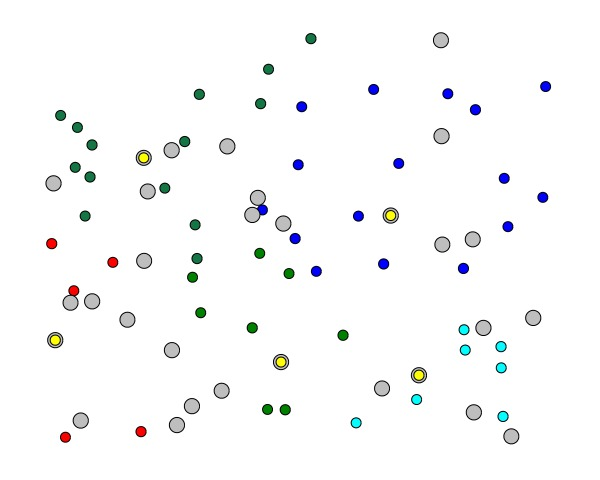
\includegraphics[scale=0.40]{graph_problem}
  \end{center}
}

\subsection{Motivation}
\begin{frame}
  When a car accident occurs, traffic congestion starts to pile up.
  This is because customers are not allowed to move their vehicles
  until the adjuster arrives.  
  The adjuster must record and determine the causes of the accident, 
  in order to move the car from the accident area and restore the flow.
  \begin{center}
    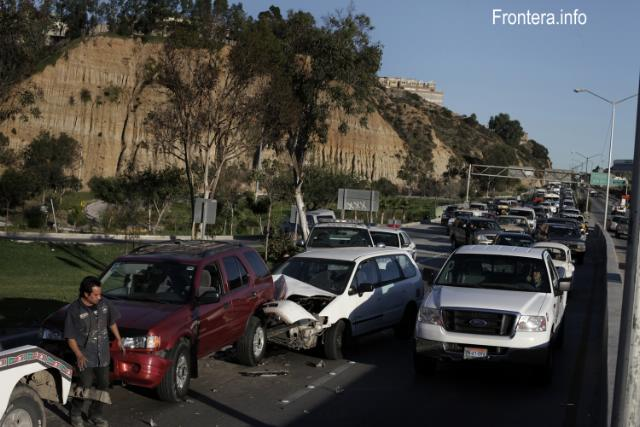
\includegraphics[scale=0.25]{389200-G}
  \end{center}
\end{frame}

\subsection{Background}
\begin{frame}[allowframebreaks]
  Richard Larson (1974) \cite{larson1974hypercube,larson1975approximating}
  proposes the Hypercube, and A-Hypercube models
  for a queuing approach for locating multiple facilities.

  James P. Jarvis (1985) \cite{jarvis1985approximating} incorporates
  location dependent service times characteristics for the A-Hypercube model,
  developing an approximation model for a spatially distributed queuing system
  under general service time assumptions.

  Berman et al. (1987) \cite{berman1987stochastic}
  formulate the Stochastic Queue p-Median problem (SQpM),
  and propose a heuristic approach for locating cooperative service facilities
  on a network.

  Goldberg et al. (1990) \cite{goldberg1990validating}
  propose a nonlinear integer programming model
  based on general service time approximation
  for spatially distributed queuing systems.

\end{frame}



\section{Models}  
% Validating and applying a model for locating emergency medical vehicles in Tucson, AZ
% Goldberg 1990

\subsection{Goldberg}

\begin{frame}
  This model is based on Goldberg's model, and it contains assignments
  variables for all posible orders.

  The following assumptions are required in the model:
  \begin{itemize}
  \item The probability that a vehicle is busy is $\rho$
    and is unaffected by the state of the system
  \item There is a strict ordering of the bases preferred for each zone
    that does not depend on the current state of the system. 
  \item All calls are answered by a vehicle originating from its base,
    not en route back to the base
  \item Different call types may have different service times
    and may or may not be included in the system objective function
  \item The arrival of calls to the system follows a stationary distribution
  \item The model is presented using a 0-queue assumption.
  \end{itemize}
  
\end{frame}


\begin{frame}
  \begin{itemize}
  \item $V$ the set of demand centers, with $|V| = n$
  \item $W$ the set of possible site for facilities, with $|W| = m$
  \item $p$ number of response units
  \item $\rho$ is the utilization of each vehicle
  \item $t_{ij}$ is the expected travel time between zone \textit{i} and base \textit{j}.
  \item $h_{ij}^{k}$ is the probability that $j$ attend client $i$ given that
    is the kth preferred.
  \item $x_j$ it there is and adjuster in node $j$
  \item $y_{ij}^k$ if the facility j, is the k-th to cover the node $i$
  \end{itemize}
\end{frame}

\begin{frame}[allowframebreaks]
  \begin{equation}
    \min \, \sum_{j=1}^{m}{\sum_{\ell=1}^{k}{\sum_{i=1}^{n}{h_{ij}^{\ell}t_{ij}y_{ij}^{\ell}}}}
  \end{equation}
  
  \begin{align}
    \sum_{j \in W}{x_j} & = p               &                                  &\\
    \sum_{j \in W}{y_{ij}^{k}} & = 1        &         \forall i \in V, k \in I &\\
    y_{ij}^{k} & \leq x_j                   & \forall i \in V,j \in W, k \in I &\\
    \sum_{k = 1}^{p}{y_{ij}^{k}} & \leq x_j &         \forall i \in V, j \in W &
  \end{align}

  \begin{align}
    y_{ij}^{k} &\leq \sum_{r}{y_{ir}^{k-1}} &  \forall (i,j,k) \mbox{ were } r \mbox{ is closer than } &j \mbox{ to } i
  \end{align}  

  \begin{align*}
    x_{j} & \in \{0,1\}      &                 \forall j &\in W\\
    y_{ij}^{k} & \in \{0,1\} & \forall i \in V,j \in W,k &\in I
  \end{align*}
\end{frame}

% A model for the Stochastic Queue p-Median Problem
% Created by Luis Maltos & Roger Rios
% 2015

\subsection{SQp-Median model}
  
\begin{frame}
  This model was developed due to the poor performance of the previous model.
  under the assumption that the probability of being served by the $\ell$th 
  adjuster is almos zero, when $\ell$ is large enough but less than $p$.
  \begin{itemize}
  \item $M$ is a large integer.
  \item $\ell$ the number of response units of importance
  \item $a_{ik}$ kth location server regarding the node $i$
  \item $x_j$ the number of adjusters in node $j$
  \item $y_{ij}^k$ if the facility j, is the k-th to cover the node $i$
  \end{itemize}

\end{frame}

\begin{frame}[allowframebreaks]
  The objective, and the equations from (2)-(5) they are practically the same,
  it had to the need of add additional variables.
  \begin{itemize}
  \item $u_{ij}$ if the adjuster located between the facility $j$, and node $i$ are less than $\ell$
  \item $v_{ij}$ if the adjuster located between the facility $j$, and node $i$ are less than $\ell$
  \end{itemize}


  \begin{align}
    \sum_{r = 1}^{k \mid a_{ik}=j}{x_{a_{ir}}} + (p-\ell) u_{ij} & \leq p & \forall i \in V, j &\in W \\
    \sum_{r = 1}^{k \mid a_{ik}=j}{x_{a_{ir}}} + M u_{ij} & \geq \ell+1   & \forall i \in V, j &\in W \\
    \sum_{k = 1}^{\ell}{y_{ij}^{k}} + M (1 - u_{ij}) & \geq x_j           & \forall i \in V, j &\in W
  \end{align}
  
  \begin{align}
    \sum_{r = 1}^{k \mid a_{i(k+1)}=j}{x_{a_{ir}}} + (p-(\ell-1)) v_{ij} & \leq p                                     & \forall i \in V, j &\in W\\
    \sum_{r = 1}^{k \mid a_{i(k+1)}=j}{x_{a_{ir}}} + M v_{ij}         & \geq \ell                                     & \forall i \in V, j &\in W\\
    \sum_{k=1}^{k}{y_{ij}^{k}} + M (1 - v_{ij} + u_{ij}) & \geq \ell - \sum_{r = 1}^{k \mid a_{i(k+1)}=j}{x_{a_{ir}}} & \forall i \in V, j &\in W\\
    \sum_{k=1}^{k}{y_{ij}^{k}} - M (1 - v_{ij} + u_{ij}) & \leq \ell - \sum_{r = 1}^{k \mid a_{i(k+1)}=j}{x_{a_{ir}}} & \forall i \in V, j &\in W\\
    y_{ij}^{k} & \leq u_{ij} + v_{ij}  &       \forall i \in V,j &\in W 
  \end{align}
  
  \begin{align*}
    x_j & \in \{0,1,\ldots,p\}         &               \forall j &\in V \\
    y_{ij}^{k} & \in \{0,1\}           & \forall i\in V,j\in W,k &\in I \\
    u_{ij},v_{ij} & \in \{0,1\}        &       \forall i \in V,j &\in W
  \end{align*}

  inspired by the results of Berman, the variable $x_j$ 
  was changed to integer variable.
\end{frame}



%\include{Experimentation}

%
\section{Results}
\subsection{Experimentation}
\begin{frame}
  All experiments were evaluated in a Lanix Spine BW
  Processor Intel Xenon, CPU E5-2867W, 3.10 GHz.
  With operative system Ubuntu 14.04.3 LTS
  The models were solved with CPLEX 12.6.0.0,
  and they were coded in C++.
\end{frame}

\begin{frame}
  Different random instances were generated
  to test the models, and verify that the solution are the same.
  For $n = 100$ were created 3 instances with $m = 20,30,40$,
  and different values of $p$, shown in the following table.
  \begin{table}
    \centerign
    \begin{tabular}{|c|c|c|}\hline
      n & m & p \\ \hline
      100 & 20 & 5-18 \\
      100 & 30 & 7-25 \\
      100 & 40 & 9,10 \\
      \hline
    \end{tabular}
  \end{table}
  
  The Model A was solved to optimality for all the values of $p$ when $m = 20$,
  for the rest of the values of $m$, could not find the optimal solution in less than one hour.

  The Model B was tested with each combination of $n,m,p$ and $\ell$ from $1,\ldots,p$.
  The results of the time of solution are shown in the following graphics,
  comparing the relation of $\frac{\ell}{p}$ versus the solution time.

\end{frame}

\begin{frame}
  Relation of $\frac{\ell}{p}$ versus the solution time.
  \begin{center}
    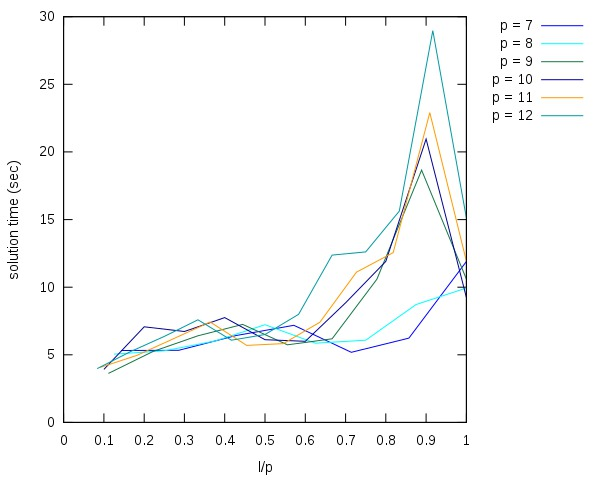
\includegraphics[scale=0.25]{grafica_01}
    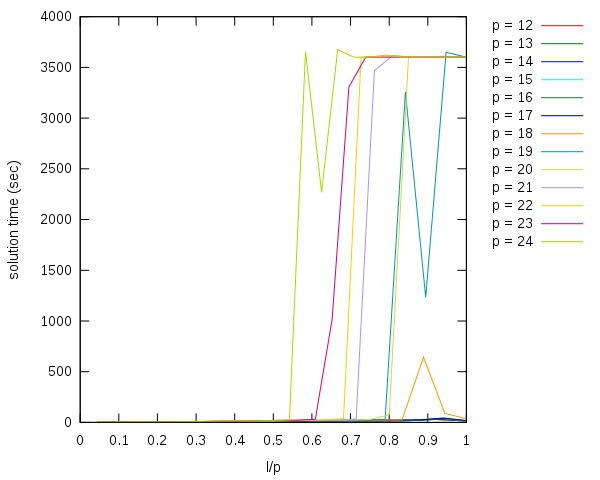
\includegraphics[scale=0.25]{grafica_02}
  \end{center}
\end{frame}

\begin{frame}

  The solution times increase drastically as $\ell$ approximates to $p$
  
  \begin{center}
    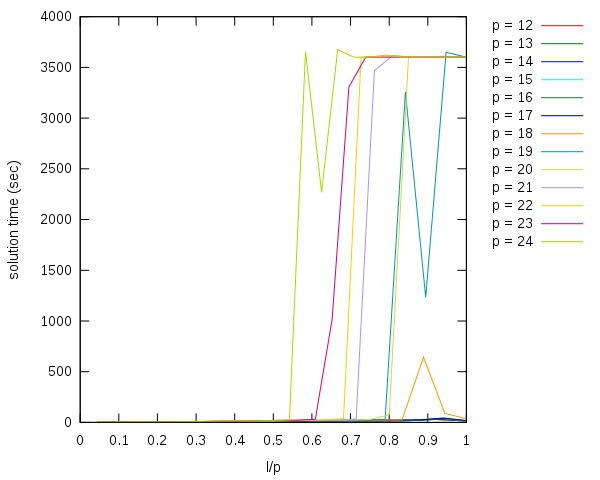
\includegraphics[scale=0.25]{grafica_02}
    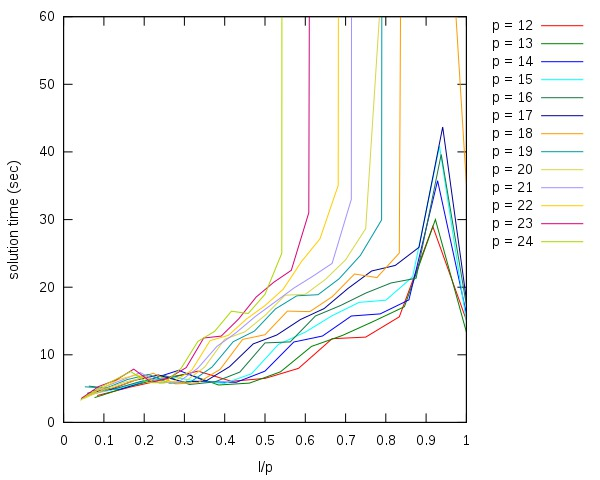
\includegraphics[scale=0.25]{grafica_03}
  \end{center}
  
\end{frame}

\begin{frame}

  For medium values of $p$, the value of the objective function does not change
  for medium/small to large values of $\ell$, were the optimal solution is obtained.

  \begin{center}
    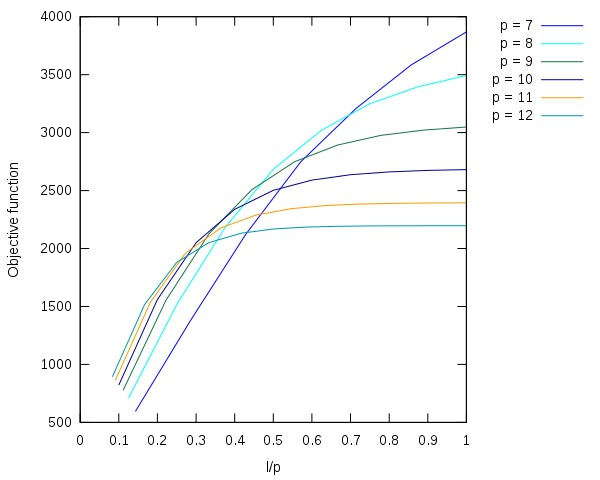
\includegraphics[scale=0.25]{grafica_04}
    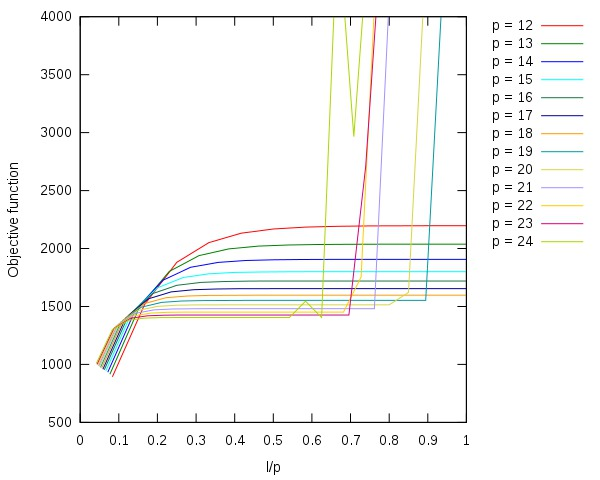
\includegraphics[scale=0.25]{grafica_05}
  \end{center}
  
\end{frame}

%% Caso 100 30 12
\frame{\begin{figure}[h!]\centering{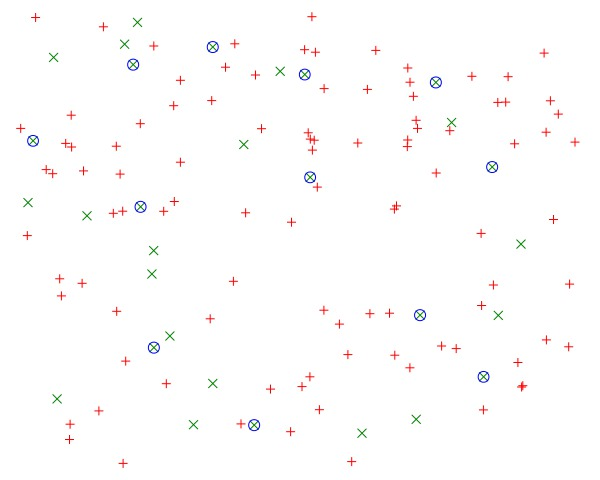
\includegraphics[scale=0.35]{Test_100_30_12_01}\caption{n = 100, m = 30, p = 12, l = 1}}\end{figure}}
\frame{\begin{figure}[h!]\centering{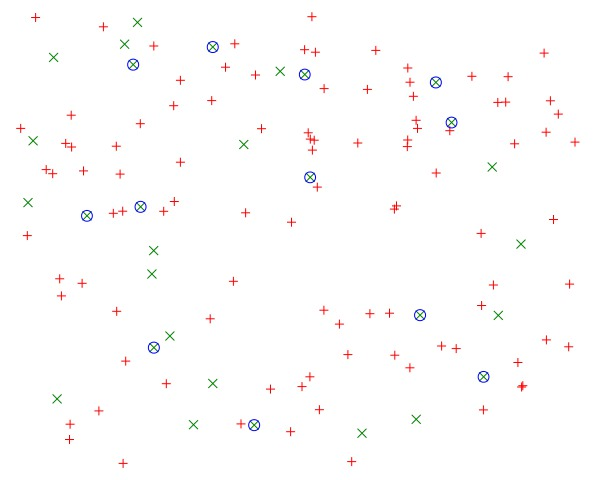
\includegraphics[scale=0.35]{Test_100_30_12_02}\caption{n = 100, m = 30, p = 12, l = 2}}\end{figure}}
\frame{\begin{figure}[h!]\centering{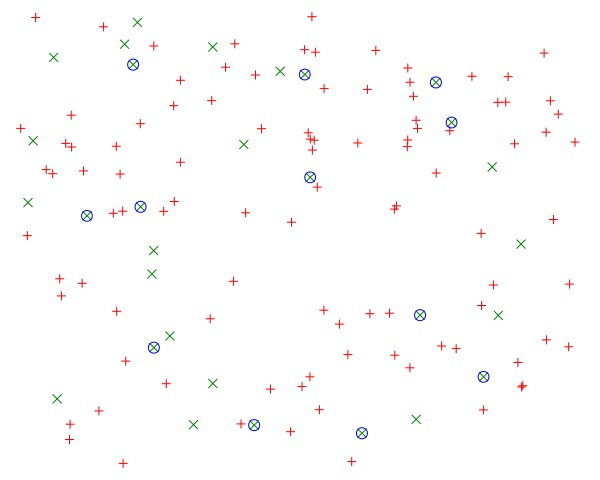
\includegraphics[scale=0.35]{Test_100_30_12_03}\caption{n = 100, m = 30, p = 12, l = 3}}\end{figure}}
\frame{\begin{figure}[h!]\centering{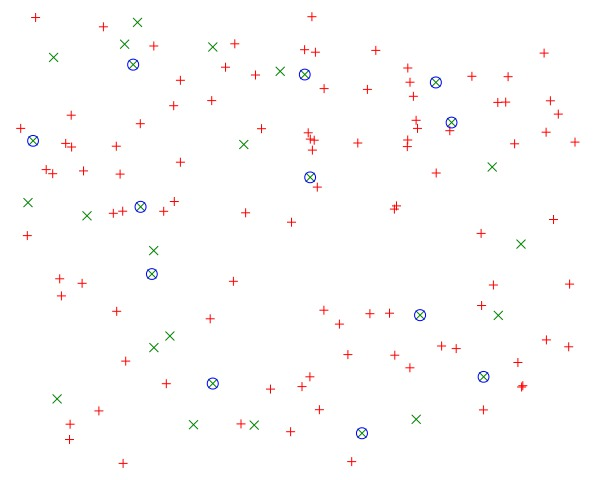
\includegraphics[scale=0.35]{Test_100_30_12_04}\caption{n = 100, m = 30, p = 12, l = 4}}\end{figure}}
\frame{\begin{figure}[h!]\centering{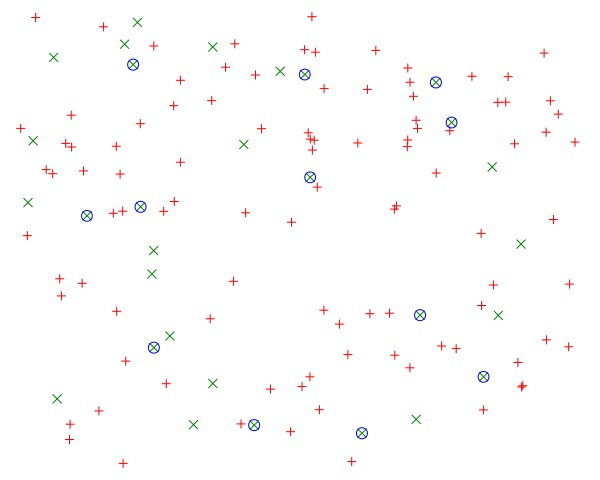
\includegraphics[scale=0.35]{Test_100_30_12_05}\caption{n = 100, m = 30, p = 12, l = 5}}\end{figure}}
\frame{\begin{figure}[h!]\centering{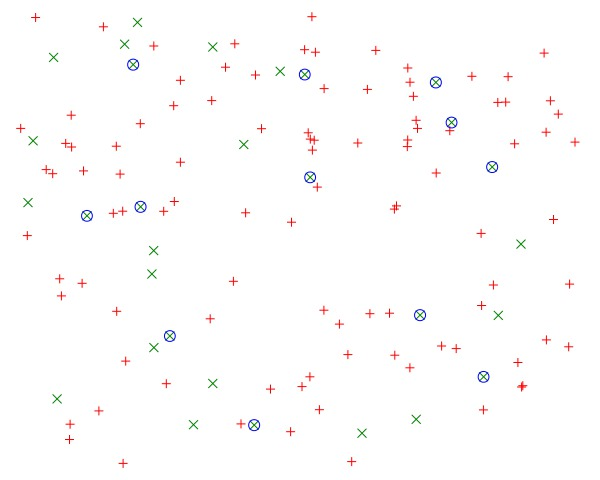
\includegraphics[scale=0.35]{Test_100_30_12_06}\caption{n = 100, m = 30, p = 12, l = 6}}\end{figure}}
\frame{\begin{figure}[h!]\centering{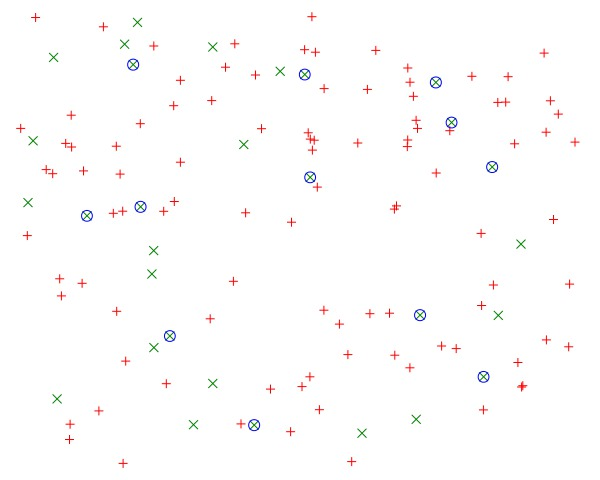
\includegraphics[scale=0.35]{Test_100_30_12_07}\caption{n = 100, m = 30, p = 12, l = 7}}\end{figure}}
\frame{\begin{figure}[h!]\centering{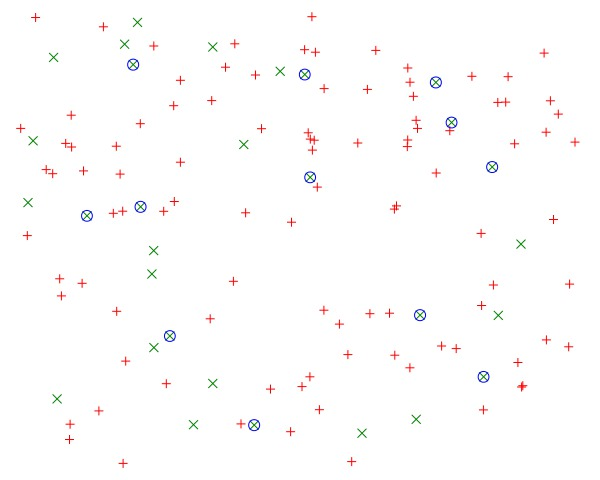
\includegraphics[scale=0.35]{Test_100_30_12_08}\caption{n = 100, m = 30, p = 12, l = 8}}\end{figure}}
\frame{\begin{figure}[h!]\centering{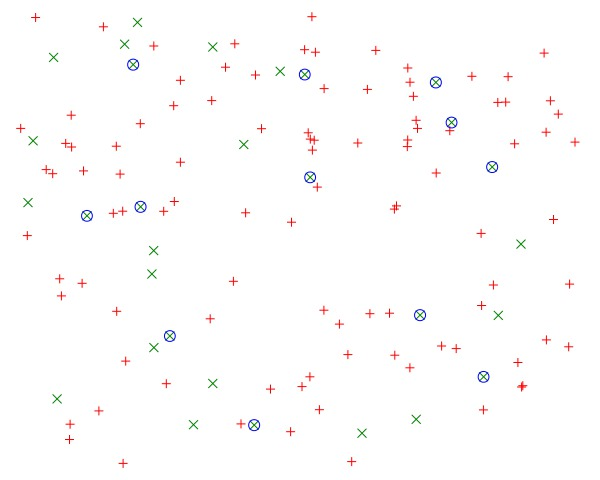
\includegraphics[scale=0.35]{Test_100_30_12_09}\caption{n = 100, m = 30, p = 12, l = 9}}\end{figure}}
\frame{\begin{figure}[h!]\centering{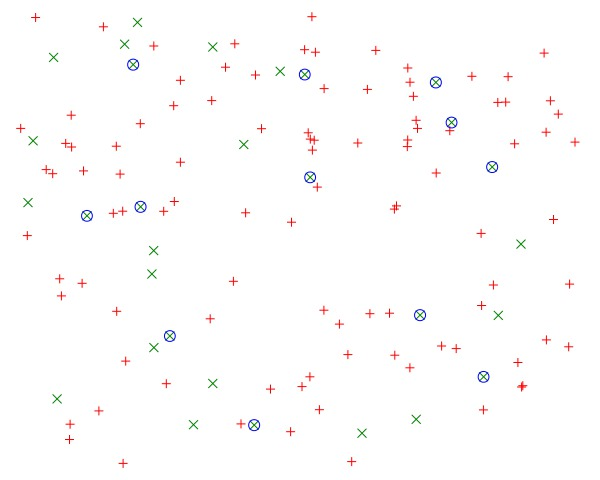
\includegraphics[scale=0.35]{Test_100_30_12_10}\caption{n = 100, m = 30, p = 12, l = 10}}\end{figure}}
\frame{\begin{figure}[h!]\centering{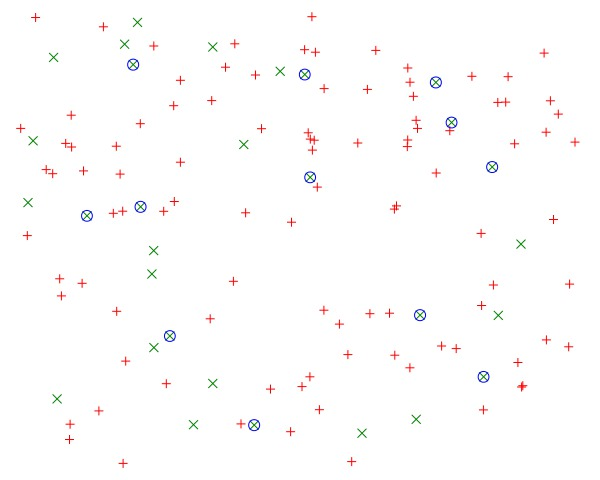
\includegraphics[scale=0.35]{Test_100_30_12_11}\caption{n = 100, m = 30, p = 12, l = 11}}\end{figure}}
\frame{\begin{figure}[h!]\centering{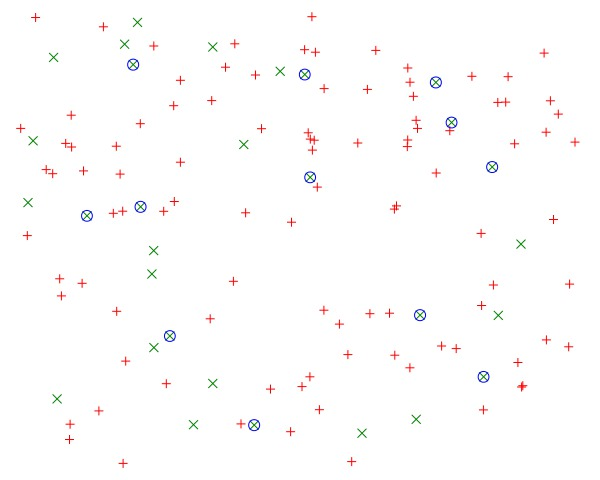
\includegraphics[scale=0.35]{Test_100_30_12_12}\caption{n = 100, m = 30, p = 12, l = 12}}\end{figure}}

\frame{\begin{figure}[h!]\centering{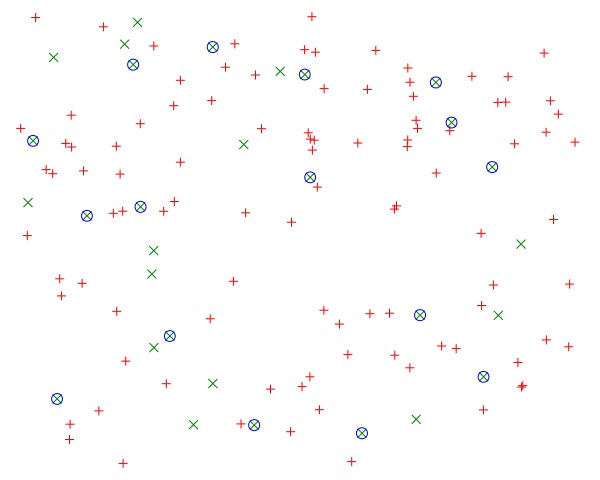
\includegraphics[scale=0.35]{Test_100_30_16_01}\caption{n = 100, m = 30, p = 16, l = 1}}\end{figure}}
\frame{\begin{figure}[h!]\centering{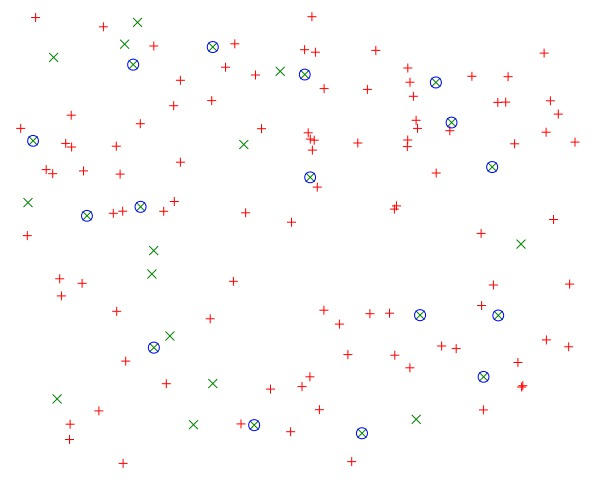
\includegraphics[scale=0.35]{Test_100_30_16_02}\caption{n = 100, m = 30, p = 16, l = 2}}\end{figure}}
\frame{\begin{figure}[h!]\centering{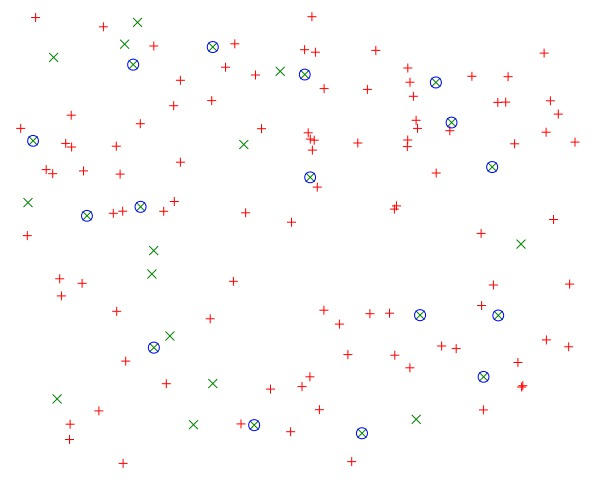
\includegraphics[scale=0.35]{Test_100_30_16_03}\caption{n = 100, m = 30, p = 16, l = 3}}\end{figure}}
\frame{\begin{figure}[h!]\centering{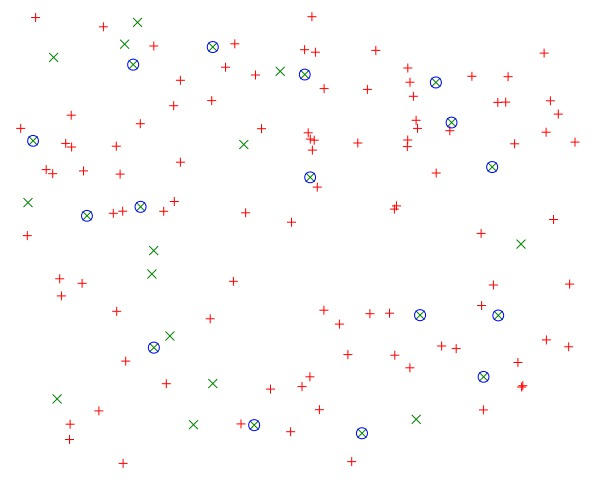
\includegraphics[scale=0.35]{Test_100_30_16_04}\caption{n = 100, m = 30, p = 16, l = 4}}\end{figure}}
\frame{\begin{figure}[h!]\centering{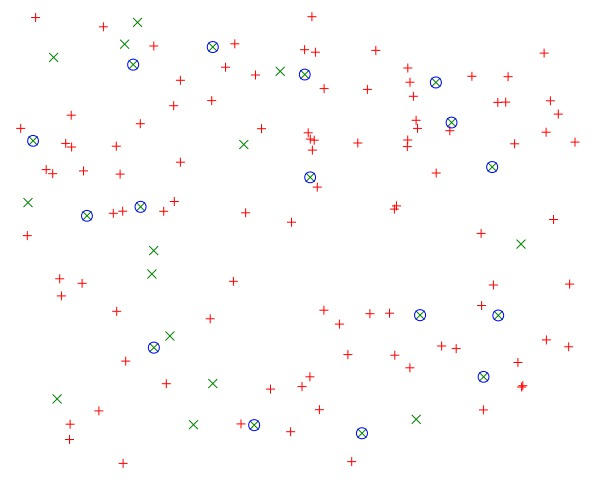
\includegraphics[scale=0.35]{Test_100_30_16_05}\caption{n = 100, m = 30, p = 16, l = 5}}\end{figure}}
\frame{\begin{figure}[h!]\centering{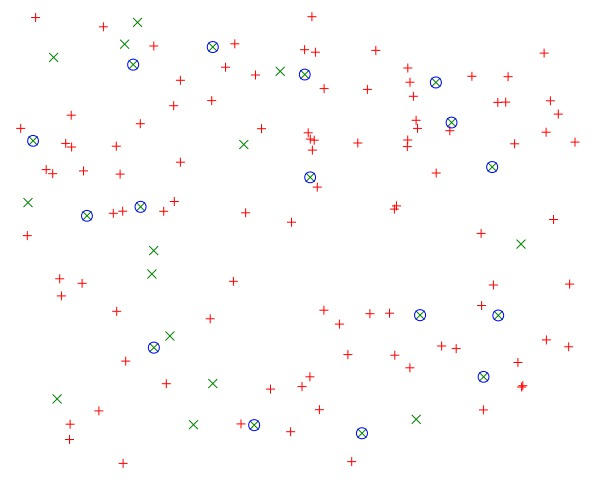
\includegraphics[scale=0.35]{Test_100_30_16_06}\caption{n = 100, m = 30, p = 16, l = 6}}\end{figure}}
\frame{\begin{figure}[h!]\centering{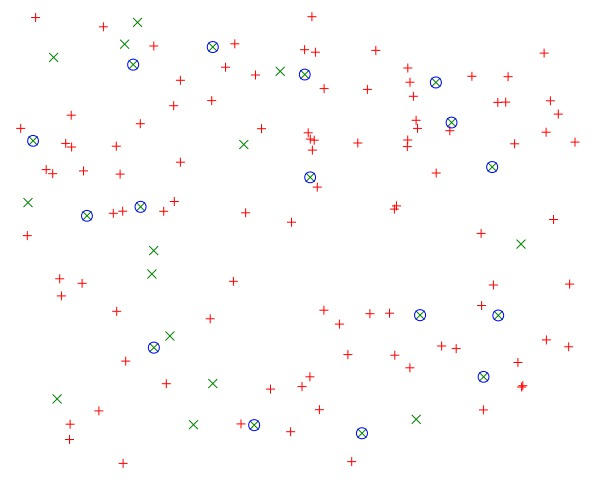
\includegraphics[scale=0.35]{Test_100_30_16_07}\caption{n = 100, m = 30, p = 16, l = 7}}\end{figure}}
\frame{\begin{figure}[h!]\centering{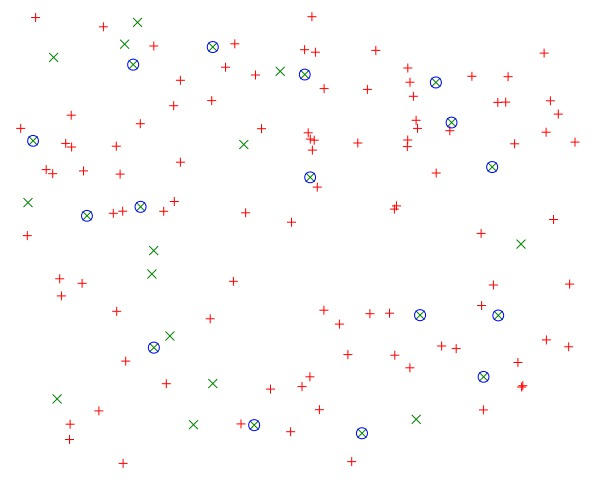
\includegraphics[scale=0.35]{Test_100_30_16_08}\caption{n = 100, m = 30, p = 16, l = 8}}\end{figure}}
\frame{\begin{figure}[h!]\centering{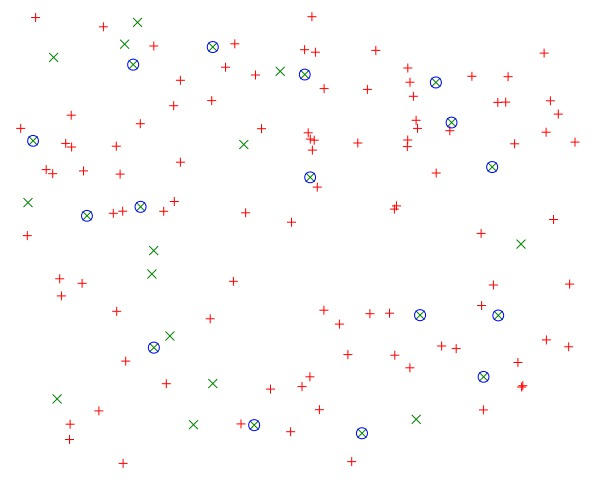
\includegraphics[scale=0.35]{Test_100_30_16_09}\caption{n = 100, m = 30, p = 16, l = 9}}\end{figure}}
\frame{\begin{figure}[h!]\centering{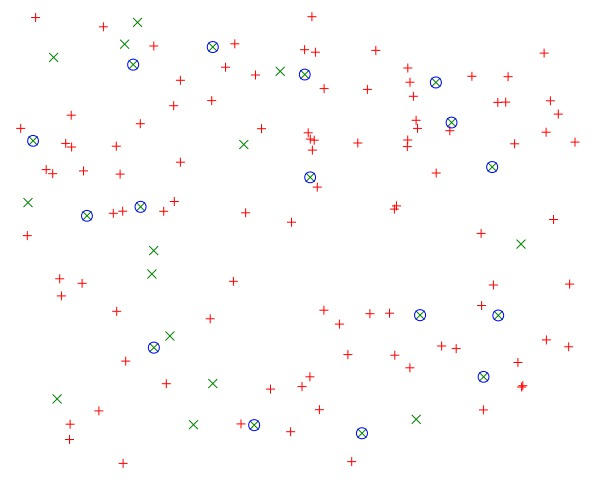
\includegraphics[scale=0.35]{Test_100_30_16_10}\caption{n = 100, m = 30, p = 16, l = 10}}\end{figure}}
\frame{\begin{figure}[h!]\centering{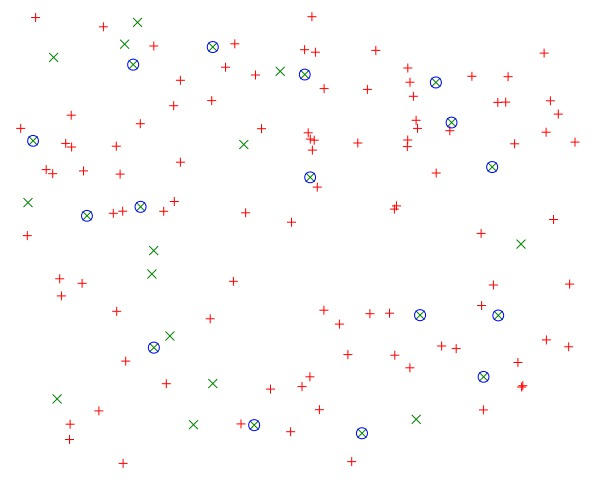
\includegraphics[scale=0.35]{Test_100_30_16_11}\caption{n = 100, m = 30, p = 16, l = 11}}\end{figure}}
\frame{\begin{figure}[h!]\centering{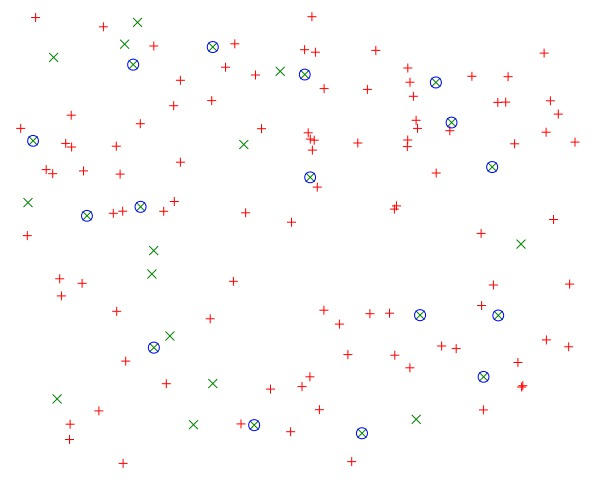
\includegraphics[scale=0.35]{Test_100_30_16_12}\caption{n = 100, m = 30, p = 16, l = 12}}\end{figure}}
\frame{\begin{figure}[h!]\centering{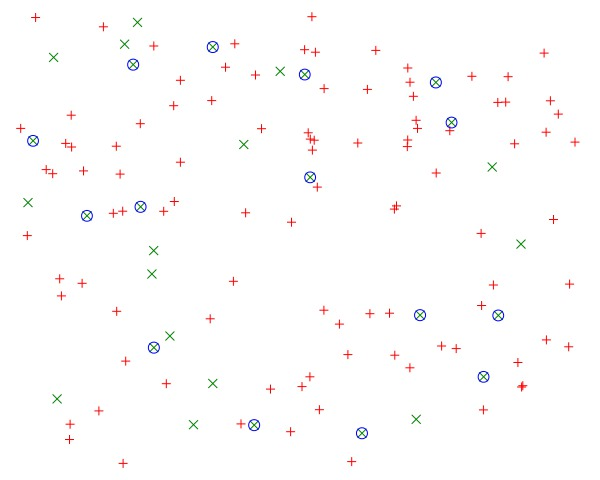
\includegraphics[scale=0.35]{Test_100_30_16_13}\caption{n = 100, m = 30, p = 16, l = 13}}\end{figure}}
\frame{\begin{figure}[h!]\centering{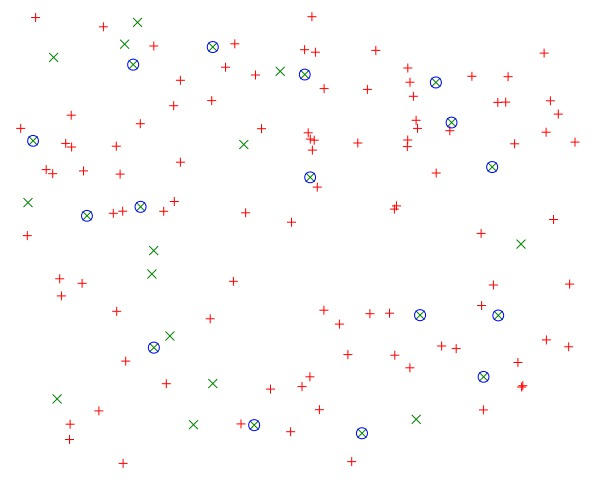
\includegraphics[scale=0.35]{Test_100_30_16_14}\caption{n = 100, m = 30, p = 16, l = 14}}\end{figure}}
\frame{\begin{figure}[h!]\centering{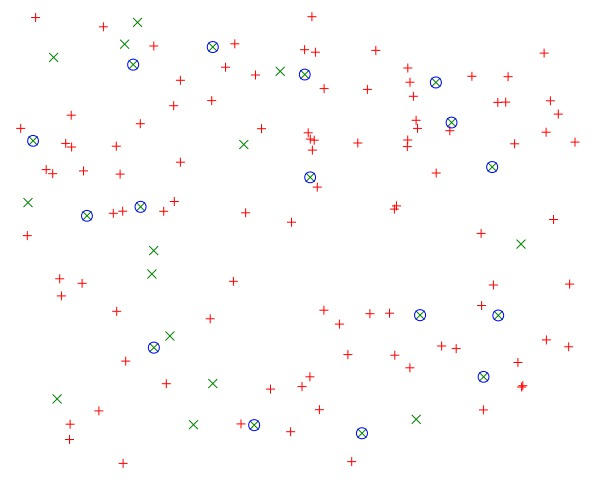
\includegraphics[scale=0.35]{Test_100_30_16_15}\caption{n = 100, m = 30, p = 16, l = 15}}\end{figure}}
\frame{\begin{figure}[h!]\centering{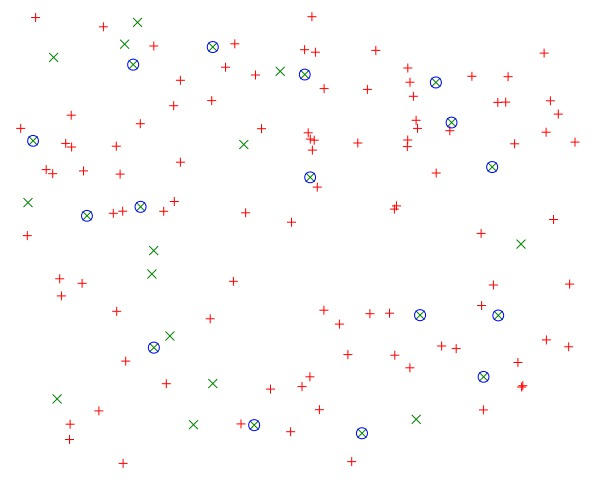
\includegraphics[scale=0.35]{Test_100_30_16_16}\caption{n = 100, m = 30, p = 16, l = 16}}\end{figure}}


%\include{Futre Wortk}


%%%
\begin{frame}[allowframebreaks]
  \frametitle<presentation>{Bibliografia}    
  \begin{thebibliography}{10}    
    \beamertemplatebookbibitems

  \bibitem{larson1974hypercube}
    Larson, Richard C,
    \emph{A hypercube queuing model for facility location and redistricting in urban emergency services},
    Computers \& Operations Research, volume 1, number 1, pages 67--95, Elsevier, 1974.
      
  \bibitem{jarvis1985approximating}
    Jarvis, James P,
    \emph{Approximating the equilibrium behavior of multi-server loss systems},
    Management Science, volume 31, number 2, pages 235--239, INFORMS, 1985.

  \bibitem{berman1987stochastic}
    Berman, Oded and Larson, RC and Parkan, Celik,
    \emph{The stochastic queue p-median problem},
    Transportation Science, volume 21, no. 3, pages 207--216, INFORMS,1987.

  \bibitem{goldberg1990validating}
    Goldberg, Jeffrey and Dietrich, Robert and Chen, Jen Ming and Mitwasi, M George and Valenzuela, Terry and Criss, Elizabeth,
    \emph{Validating and applying a model for locating emergency medical vehicles in Tuczon, AZ},
    European Journal of Operational Research, volume 49, no. 3, pages 308--324, Elsevier, 1990.

%  \bibitem{marianov1998probabilistic}
%    Marianov, Vladimir and Serra, Daniel,
%    \emph{Probabilistic maximal covering location-allocation models for congested systems}
%    Journal of Regional Science, volume 38, number 3, pages 401--424, Wiley Online Library,1998.

%  \bibitem{rajagopalan2008multiperiod}
%    Rajagopalan, Hari K and Saydam, Cem and Xiao, Jing,
%    \emph{A multiperiod set covering location model for dynamic redeployment of ambulances},
%    Computers Operations Research, volume 35, no. 3, pages 814--826, Elsevier, 2008

%  \bibitem{pereira2015hybrid}
%    Pereira, Marcos A and Coelho, Leandro C and Lorena, Luiz AN and De Souza, Ligia C,
%    \emph{A hybrid method for the Probabilistic Maximal Covering Location--Allocation Problem},
%    Computers \& Operations Research, volume 57, pages 51--59, Elsevier, 2015.

  \end{thebibliography}
\end{frame}

\end{document}
